\documentclass[border=4pt]{standalone}
\usepackage{amsmath,amssymb,tikz}
\usetikzlibrary{arrows.meta,calc,matrix,positioning}
\definecolor{figB}{RGB}{31,90,166}\definecolor{figR}{RGB}{176,48,48}\definecolor{figG}{RGB}{46,125,50}\definecolor{figO}{RGB}{214,120,20}
\begin{document}
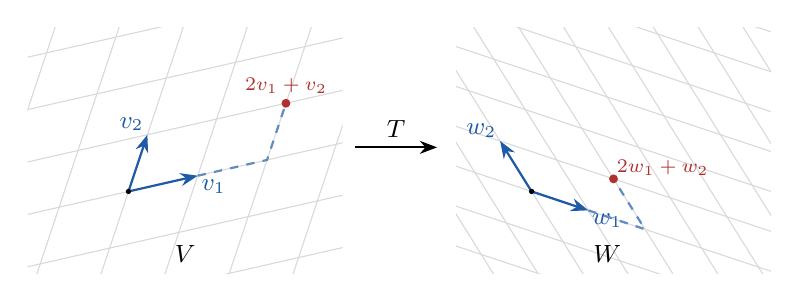
\begin{tikzpicture}[scale=0.8,>={Stealth[length=2.2mm]}]
% V with basis v1=(1.1,0.25), v2=(0.3,0.9)
\begin{scope}
\clip (-1.6,-1.3) rectangle (3.4,2.6);
\foreach \s in {-8,...,8} \draw[black!15,thin] ({\s*1.1-8*0.3},{\s*0.25-8*0.9})--({\s*1.1+8*0.3},{\s*0.25+8*0.9});
\foreach \t in {-4,...,5} \draw[black!15,thin] ({-8*1.1+\t*0.3},{-8*0.25+\t*0.9})--({8*1.1+\t*0.3},{8*0.25+\t*0.9});
\end{scope}
\draw[->,thick,figB] (0,0)--(1.1,0.25) node[below right,font=\small,inner sep=1pt]{$v_1$};
\draw[->,thick,figB] (0,0)--(0.3,0.9) node[above left,font=\small,inner sep=1pt]{$v_2$};
\draw[figB!70,dashed,thick] (1.1,0.25)--(2.2,0.5)--(2.5,1.4);
\fill[figR] (2.5,1.4) circle (2pt) node[above,font=\scriptsize]{$2v_1+v_2$};
\fill (0,0) circle (1.2pt);
\node[font=\small] at (0.9,-1.0) {$V$};
\draw[->,thick] (3.6,0.7)--(4.9,0.7) node[midway,above,font=\small]{$T$};
% W with w1=(0.9,-0.3), w2=(-0.5,0.8)
\begin{scope}[xshift=6.4cm]
\begin{scope}
\clip (-1.2,-1.3) rectangle (3.8,2.6);
\foreach \s in {-8,...,8} \draw[black!15,thin] ({\s*0.9+8*0.5},{-\s*0.3-8*0.8})--({\s*0.9-8*0.5},{-\s*0.3+8*0.8});
\foreach \t in {-8,...,8} \draw[black!15,thin] ({-12*0.9-\t*0.5},{12*0.3+\t*0.8})--({12*0.9-\t*0.5},{-12*0.3+\t*0.8});
\end{scope}
\draw[->,thick,figB] (0,0)--(0.9,-0.3) node[below right,font=\small,inner sep=1pt]{$w_1$};
\draw[->,thick,figB] (0,0)--(-0.5,0.8) node[above left,font=\small,inner sep=1pt]{$w_2$};
\draw[figB!70,dashed,thick] (0.9,-0.3)--(1.8,-0.6)--(1.3,0.2);
\fill[figR] (1.3,0.2) circle (2pt) node[above right,font=\scriptsize,inner sep=1pt]{$2w_1+w_2$};
\fill (0,0) circle (1.2pt);
\node[font=\small] at (1.2,-1.0) {$W$};
\end{scope}
\end{tikzpicture}
\end{document}
